\section{Das Magnetische Feld}

\subsection{Energie und Kraft im magnetischen Feld}
\textbf{Energiedichte:}
$\boxed{w_m=\int_0^B{\vec{H}\cdot d\vec{B}}}$ (Allgemein)
$\qquad\boxed{w_m=\frac{1}{2}B\cdot H}$ (homog. Feld) $\qquad [w_m]=\frac{J}{m^3}$\\

\textbf{Energie:}
$\boxed{W_m = \frac{1}{2} \cdot L \cdot I^2=\frac{1}{2}\cdot N \cdot I \cdot
\Phi \; \text{ or } \; W_m=\frac{1}{2} \int_V \vec H \cdot
\vec B \cdot dV}$ (Allg.)
$\quad\boxed{W_m=w_m \cdot V=\frac{1}{2} \cdot B \cdot H \cdot V}$ (homog. Feld)\\
\parbox{5cm}{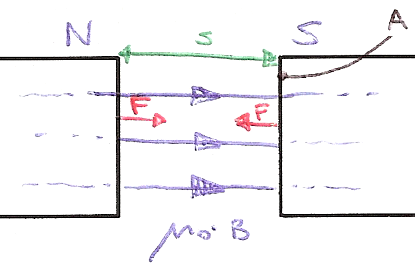
\includegraphics[width=4cm]{./pics/m-kraft-mfeld.png}}
\parbox{13cm}{	
	Die Kraft auf Grenzfl�chen ist stets so gerichtet, dass sie die Induktivit�t
	zu vergr�ssern sucht. Das heisst immer vom ferromagnetischen Material zur
	nichtferromagnetischen Umgebung (z.B. Luft). Prinzip der virtuellen
	Verschiebung:\\
	$$\boxed{F = \left| \frac{\mathrm dW_m}{\mathrm ds} \right| = \frac{1}{2} I^2 \cdot \frac{\mathrm dL}{\mathrm ds} 
	\qquad oder \qquad  F = \frac{1}{2} \cdot B \cdot H \cdot A=\frac{1}{2} \cdot
	\frac{B^2}{\mu} \cdot A \text{ (f�r } \mu_{rFe} \gg  \text{ 1)}}$$ }

\newpage